\documentclass[mathserif,18pt,xcolor=table]{beamer}
\usepackage{amsmath}
\usepackage{amssymb}
\usepackage{bbm}
\usepackage{ulem}
\usepackage{feynmp-auto}
%\usepackage{slashed}
\usepackage[absolute,overlay]{textpos}
\usepackage{graphicx}
\usepackage{listings}
\usepackage{epsfig}
\usepackage{hyperref}
\usepackage{tikz}
\usetikzlibrary{calc}
\usepackage{enumerate}
%\usepackage{fixltx2e} % buggy
\usepackage[compatibility=false]{caption}
\usepackage{subcaption} % doesn't work with subfigure
%\usepackage{pdfpages}
\usepackage{setspace}
\usepackage{verbatim}
\usepackage{physics}
%\usepackage{siunitx}

\DeclareRobustCommand{\orderof}{\ensuremath{\mathcal{O}}}

\definecolor{dukeblue}{RGB}{0,0,156}
\definecolor{dukedarkblue}{RGB}{0,26,87}
\definecolor{dukeblack}{RGB}{79,79,79}
\definecolor{dukegray}{RGB}{79,79,79}
\definecolor{dukesecbrown}{RGB}{217,200,158}
\definecolor{dukesecblue}{RGB}{127,169,174}
\mode<presentation> {
  \usetheme{Boadilla}  
  \setbeamercovered{invisible}
  \setbeamertemplate{navigation symbols}{}  
  \setbeamertemplate{frametitle}[default][center]
  \setbeamertemplate{bibliography item}{\insertbiblabel}
  \setbeamerfont{frametitle}{series=\bfseries,parent=structure}
  \setbeamerfont{subtitle}{size=\scriptsize,series=\bfseries,parent=structure}
  \setbeamerfont{author}{size=\scriptsize,parent=structure}
  \setbeamerfont{institute}{size=\small,series=\bfseries,parent=structure}
  \setbeamerfont{date}{size=\scriptsize,parent=structure}
  \setbeamerfont{footline}{size=\tiny,parent=structure}
  \setbeamercolor{normal text}{bg=white,fg=dukeblack}
  \setbeamercolor{structure}{fg=dukeblue}
  \setbeamercolor{alerted text}{fg=red!85!black}
  \setbeamercolor{item projected}{use=item,fg=black,bg=item.fg!35}
  \setbeamercolor*{palette primary}{use=structure,fg=white, bg=dukeblue}
  \setbeamercolor*{palette secondary}{use=structure,bg=dukedarkblue,fg=white}
  \setbeamercolor*{framesubtitle}{fg=dukegray}
  \setbeamercolor*{block title}{parent=structure,fg=black,bg=dukeblue}
  \setbeamercolor*{block body}{fg=black,bg=dukeblack!10}
  \setbeamercolor*{block title alerted}{parent=alerted text,bg=black!15}
  \setbeamercolor*{block title example}{parent=example text,bg=black!15}
}

\makeatletter
\setbeamertemplate{footline}{
  \leavevmode
  \hbox{%
    \begin{beamercolorbox}[wd=.333333\paperwidth,ht=2.25ex,dp=1ex,center]{author in head/foot}%
      \usebeamerfont{author in head/foot}\insertshortauthor%
    \end{beamercolorbox}%
    \begin{beamercolorbox}[wd=.333333\paperwidth,ht=2.25ex,dp=1ex,center]{title in head/foot}%
      \usebeamerfont{title in head/foot}\insertshorttitle%
    \end{beamercolorbox}%
    \begin{beamercolorbox}[wd=.333333\paperwidth,ht=2.25ex,dp=1ex,right]{date in head/foot}%
      \usebeamerfont{date in head/foot}\insertshortdate{}\hspace*{2em}%
      \insertframenumber{} / \inserttotalframenumber\hspace*{2ex}%
%      \insertframenumber{} / 11\hspace*{2ex}% TODO hard code to page number before backup!!
    \end{beamercolorbox}}%
  \vskip0pt%
}
\makeatother


\AtBeginSection{\frame{\sectionpage}}


\defbeamertemplate{section page}{mine}[1][]{%
  \begin{centering}
    {\usebeamerfont{section name}\usebeamercolor[fg]{section name}#1}
    \vskip1em\par
    \begin{beamercolorbox}[sep=12pt,center]{part title}
      \usebeamerfont{section title}\insertsection\par
    \end{beamercolorbox}
  \end{centering}
}


\usepackage[protrusion=true,expansion=true]{microtype}
\usepackage{amsmath}
\renewcommand*{\thefootnote}{\fnsymbol{footnote}}
\title[Group Project 2]{Group Project 2\newline Percolation}
\author[Xu, Epland, Li, Cohen]{{\small Yuanyuan Xu, Matthew Epland, Xiaqing Li, Wesley Cohen}}
\institute{Duke University}
%\date{\today}
\date{April 8, 2016}
\hypersetup{
    breaklinks,
    baseurl       = http://,
    pdfborder     = 0 0 0,
    pdfpagemode   = UseNone,% do not show thumbnails or bookmarks on opening
    pdfstartpage  = 1,
    bookmarksopen = true,
    bookmarksdepth= 2,% to show sections and subsections
    pdfauthor     = {\@author},
    pdftitle      = {\@title},
    pdfsubject    = {},
    pdfkeywords   = {}}

\titlegraphic{
\includegraphics[height=2cm]{logos/duke_logo.pdf}}

% Point to nice top level directory
\graphicspath{{../output/plots_for_paper/}}

\begin{document}

\beamertemplateballitem
\frame{\titlepage}
\addtobeamertemplate{frametitle}{}{}

\


\begin{frame}
	\frametitle{Introduction -- Part A}
	Percolation transition on a $N\times N$ lattice:
	\begin{itemize}
		\item Sites are subsequently and randomly occupied
		\item A cluster -- a collection of interconnection occupied sites
		\begin{itemize}
			\item A \textbf{spanning cluster} touches all four edges of the lattice
			\item Percolation transition -- when the spanning cluster occurs
		\end{itemize}
		\item Occupation probability: 
			\begin{equation}
			p=\frac{\text{number of occupied sites}}{N^2}
			\end{equation}
		\begin{itemize}
			\item At the \textbf{critical concentration $p_c$} percolation transition occurs
		\end{itemize}
	\end{itemize}
\end{frame}


\begin{frame}
	\frametitle{Union-Find Algorithms}
	\begin{itemize}
		\item Data structure
			\begin{itemize}
			\item Integer array {\tt label[i]} of size $N\times N$.
			\item interpretation: {\tt p} and {\tt q} are connected if they have the same label.
			\end{itemize}
		\item Find: Check if {\tt p} and {\tt q} have the same label.
		\item Union: To merge components containing {\tt p} and {\tt q}, change all entries with {\tt label[p]} to {\tt label[q]}.
	\end{itemize}
\end{frame}


\begin{frame}
	\frametitle{Percolation}
	\begin{itemize}
		\item Initialization \qquad
			\begin{tabular}{|l|c|r|}
				\hline
				0 & 0 & 0 \\ \hline
				0 & 0 & 0 \\ \hline
				0 & 0 & 0 \\	 \hline
			\end{tabular}
		\item Generate a random sequence from 0 to $N^2-1$:\\
			\qquad {\tt arr = shuffle([0, 1, 2,..., N*N-1])}
		\item Occupy a site given by {\tt arr[i]}.
		\item Union: Choose a common unique label and update {\tt label}.
		\item Percolation
			\begin{itemize}
				\item Data structure: TreeSet.
				\item $S = \{{\mathrm{Edge}_{1}}\} \cap \{{\mathrm{Edge}_{2}}\} \cap \{{\mathrm{Edge}_{3}}\} \cap \{{\mathrm{Edge}_{4}}\} - \{0 \}$
				\item $
						S = \begin{cases}
 								\O & \qquad \text{unconnected,}\\
 								\{x\} & \qquad \text{connected}, x \text{ is the same label.}
 							\end{cases}
					  $
			\end{itemize}
		\item \href{run:movie.avi}{Animation}
	\end{itemize}
\end{frame}


\begin{frame}
	\frametitle{Extract $p_c$ of infinitely large 2D square lattice}
	\begin{itemize}
		\item Determine the value of $p_c$ for 2D square lattice of different lengths \\
		 \begin{itemize}
			\item $N= 5, 10, 15, 20, 30, 50, 80$		
		\end{itemize}
		 \bigskip
		 \item For each lattice size: average the results for 50 different simulations
		 \bigskip
		 \item Plot $p_c(N^{-1})$ to extrapolate to the infinite lattice limit
		 \begin{itemize}
		 	\smallskip
			\item $N^{-1}\rightarrow 0,\  p_c \rightarrow p_c \  \textit{of infinitely large lattice}$	
		\end{itemize}
	\end{itemize}
\end{frame}


\begin{frame}
	\frametitle{Resutls}
	\begin{figure}
  	\centering
  	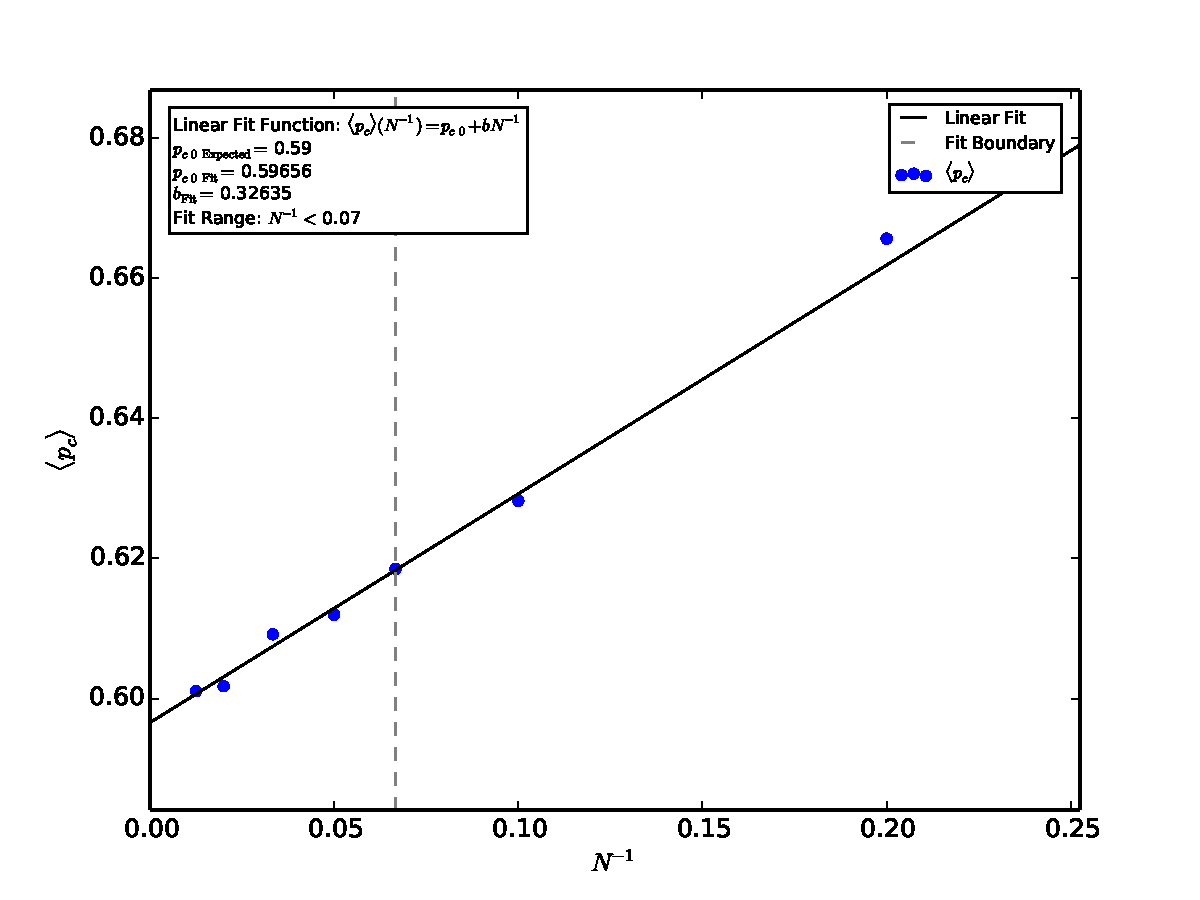
\includegraphics[width=0.9\textwidth]{../output/dev/pc_ave_vs_InverseN.pdf}
	\end{figure}
\end{frame}


\begin{frame}
	\frametitle{Introduction -- Part B}
	Fraction of sites in percolating cluster
	\begin{itemize}
		\item Definition:
			\begin{equation}
			F(p>p_c)=\frac{\text{number of sites in spanning cluster}}{\text{number of occupied sites}}
			\end{equation}
		\item $F$ near $p_c$ satisfies power law:
			\begin{equation}
			F=F_0(p-p_c)^\beta
			\end{equation}
		\item Extract $\beta$
			\begin{itemize}
				\item Linear fitting on the log-log scale plot
			\end{itemize}
	\end{itemize}
\end{frame}


\begin{frame}
	\frametitle{Resutls}
	\begin{figure}
  	\centering
  	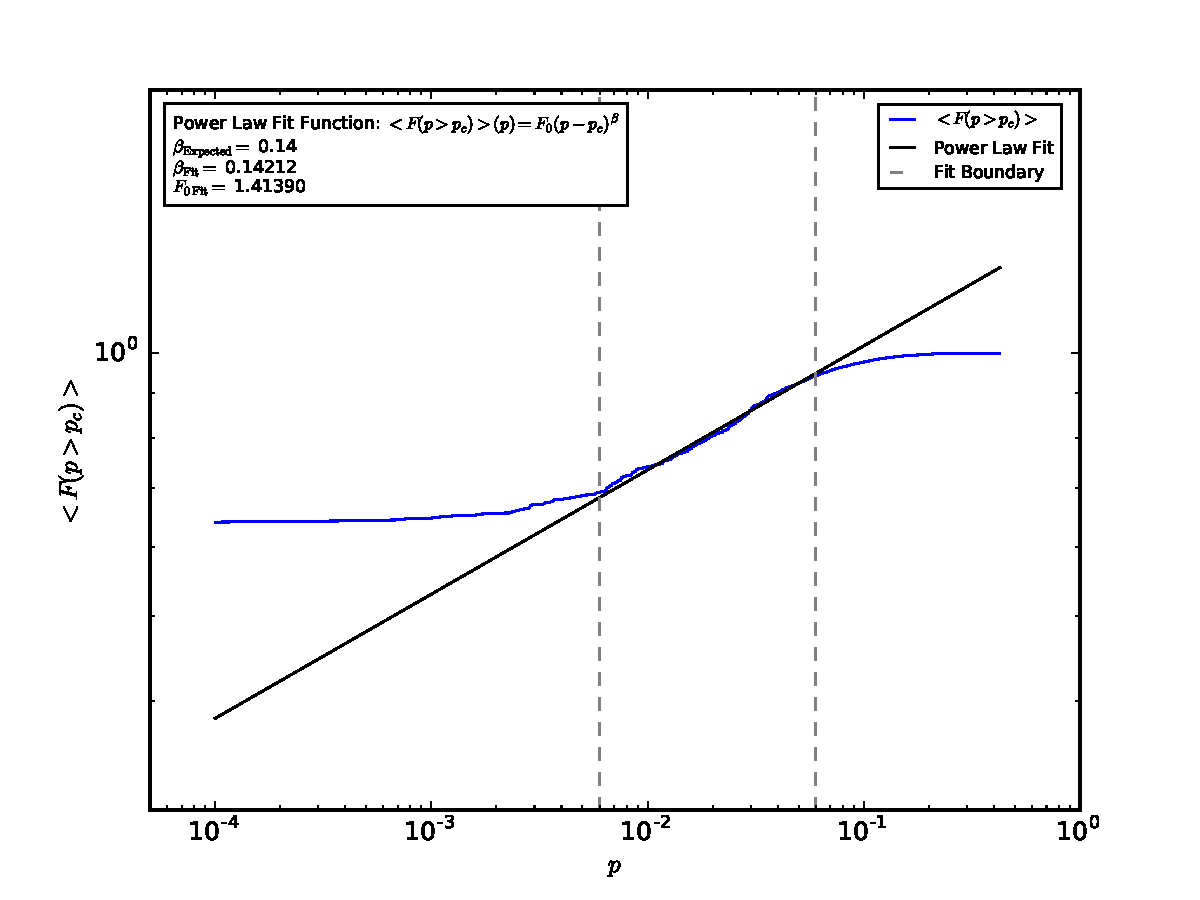
\includegraphics[width=0.9\textwidth]{../output/dev/F_ave_vs_p.pdf}
	\end{figure}
\end{frame}



\end{document}
%%%%%%%%%%%%%%%%%%%%%%%%%%%%%%%%%%%%%%%%%%%%%%%%%%%%%%%%%%%%%%%%%%%%

% Backup
\begin{frame}
    \begin{center}
    \usebeamerfont{frametitle}Backup
    \end{center}
\end{frame}

% bib
\begin{frame}%[allowframebreaks]
        \frametitle{References}
	\bibliographystyle{../bib_files/atlasBibStyleWoTitle}
{\scriptsize
        \bibliography{../bib_files/my_bib.bib}
}
\end{frame}


